\documentclass{agujournal2019}
\usepackage{url}
\usepackage{lineno}
\usepackage[inline]{trackchanges}
\usepackage{soul}
\linenumbers
\draftfalse

\journalname{Earth's Future}

\begin{document}

\title{The Global Sparsity and Regulatory Rigidity of Freshwater Fecal Indicator Bacteria Monitoring}

\authors{[Author One]\affil{1}, [Author Two]\affil{2}}

\affiliation{1}{[Affiliation one --- to be completed]}
\affiliation{2}{[Affiliation two --- to be completed]}

\correspondingauthor{[Corresponding Author]}{[corresponding author contact --- to be completed]}

\begin{keypoints}
\item We harmonized 5.3 million freshwater fecal indicator bacteria measurements from ten public sources into one global dataset
\item Openly shared monitoring is concentrated in the United States Europe and Canada revealing a data sharing gap as much as a collection gap
\item Only about seven percent of monitored sites are sampled often enough to capture the rapid changes in fecal contamination
\end{keypoints}

\begin{abstract}
Fecal indicator bacteria, especially \textit{Escherichia coli}, are the primary tool used worldwide to judge whether inland fresh waters are safe from waterborne pathogens, yet the monitoring record that underpins these decisions has never been characterized at a harmonized global scale. We compiled, harmonized, and analyzed 5{,}314{,}791 freshwater fecal indicator observations from ten public sources, standardized to a common schema, indicator set, and unit. Two structural weaknesses emerge. First, openly shared data are spatially unequal: the United States, Europe, and Canada account for roughly 89\% of records, while much of the Global South is sparse and large monitoring nations are absent from open repositories, indicating that apparent data scarcity is in part an open-data sharing barrier rather than an absence of monitoring. Second, the record is temporally rigid: only about 7\% of multi-sample sites are sampled at a daily or near-daily frequency, while contamination is a transient, weather-driven condition. Using the rare high-frequency sites, including three contrasting case studies, we show that low-frequency sampling misrepresents safety in both episodically and chronically contaminated waters. We argue for wider adoption of open-data practices and for higher-frequency, event-based, and predictive monitoring to make fecal indicator data actionable for public health. Key uncertainties include uneven coverage of non-\textit{E. coli} indicators, a geographic bias of high-frequency sites toward North America and Europe, and an approximate unit conversion between enumeration methods.
\end{abstract}

\section*{Plain Language Summary}
Bacteria such as \textit{E. coli} are measured around the world to tell whether rivers and lakes are safe for swimming and for drinking-water supply. We gathered more than five million of these measurements from ten public sources in many countries and combined them into a single comparable dataset. We found two problems. First, almost all of the freely shared data come from the United States, Europe, and Canada; many other countries monitor their waters but do not publish the results in open, reusable form, so the world looks emptier of data than it really is. Second, most places are tested too infrequently --- often only monthly or a few times a year --- to catch the short bursts of pollution that follow rainfall and that pose the greatest health risk. At the few sites tested almost daily, we show that infrequent testing gives a misleading picture of safety, both at beaches that are usually clean and at rivers that are chronically polluted. Making water-quality data more openly shared, and testing more frequently where it matters, would help protect public health.

\section{Introduction}

Fecal indicator bacteria, and \textit{Escherichia coli} in particular, are the primary tool used worldwide to judge whether fresh waters are safe from waterborne pathogens. The public-health stakes are large: inadequate water, sanitation, and hygiene remain responsible for a substantial global disease burden \cite{prssustn2014burden,prssstn2019burden,wolf2023burden}, fecal contamination of drinking water is widespread across low- and middle-income settings \cite{bain2014fecal,bain2014global}, and contact with fecally contaminated recreational water is an established cause of gastrointestinal and other illness \cite{gerdes2023estimating,wade2022health,zmirou2003risks}. Because directly enumerating the many waterborne pathogens is impractical for routine monitoring, agencies instead measure culturable indicator organisms whose presence signals fecal contamination. A long line of epidemiological studies has linked indicator concentrations to swimmer illness and established \textit{E. coli} and intestinal enterococci as the standard indicators for fresh and marine waters, respectively \citeA{cabelli1982swimmingassociated}; subsequent reviews and cohort studies refined these relationships \cite{prss1998review,wade2003environmental,wade2005rapidly,wade2010rapidly}, and \textit{E. coli} is widely regarded as the most reliable bacterial indicator of fecal contamination in fresh water \cite{edberg2000escherichia,boehm2014enterococci,korajkic2018relationships}. These relationships underpin regulatory thresholds such as the United States Environmental Protection Agency recreational criteria and the European Bathing Water Directive \cite{epa2012recreational,eu2006bathing,who2021recreational,boehm2008sea}.

Despite this central role, the global record that underpins freshwater safety decisions has never been assembled and characterized at a harmonized, global scale. Monitoring data are dispersed across dozens of national and supranational portals with incompatible schemas, units, and indicator vocabularies. A growing body of work aggregates water-quality observations to enable large-sample analysis: in the United States, the Water Quality Portal unifies federal, state, and tribal records \cite{read2017water}, although reusing such multi-source data requires substantial harmonization and quality control \cite{sprague2017challenges,bousquin2024harmonizewq}. At continental to global scale, compilations such as AquaSat, the Global River Chemistry database, the Global River Water Quality Archive, large-sample chemistry extensions of catchment datasets, and global salinity syntheses have assembled physical and chemical variables for thousands of sites \cite{ross2019aquasat,hartmann2014brief,virro2021grqa,sterle2024camelschem,thorslund2020global}, and recent work has begun to argue for global microbial water-quality data infrastructure \cite{rose2023global}. These resources are invaluable, but they are typically organized around water chemistry or single-nation coverage and do not characterize the spatial sharing structure or the temporal sampling cadence of fecal indicators specifically.

These two dimensions matter because fecal contamination is a transient, weather-driven condition. Numerous site studies document that fecal indicator concentrations vary by orders of magnitude over hours to days, exhibiting diurnal cycles, rainfall- and runoff-driven spikes, and rapid sunlight-driven decay \cite{whitman2004escherichia,whitman2004solar,traister2006variability,meays2006diurnal,desai2013escherichia,nguyen2022fecal}. This variability makes infrequent grab samples unreliable for classifying recreational safety \cite{kim2004public}, and it has motivated high-frequency sampling campaigns and statistical or data-driven nowcasting models that predict water quality from rainfall, turbidity, and discharge \cite{searcy2023highfrequency,searcy2021day,heasley2021systematic}. Regulatory thresholds, however, are defined for compliance statistics and implicitly assume representative sampling --- an assumption that weekly, monthly, or quarterly designs, often confined to a summer bathing season, routinely violate.

A complementary literature helps interpret why openly shared data are so unevenly distributed. The FAIR principles articulate norms for findable, accessible, interoperable, and reusable data \cite{wilkinson2016fair}, yet technical, institutional, and social barriers impede open sharing of water-quality and other environmental monitoring data \cite{brasier2017barriers,sugg2021social,hazell2023sociotechnical,heacock2022enhancing}, and monitoring capacity itself varies systematically with national development and the flow of information through regulatory programs \cite{kirschke2020capacity,kumpel2020data}. Together these dynamics imply that an apparent absence of data in global repositories often reflects where data are \emph{shared} rather than where they are \emph{collected}.

Here we compile, harmonize, and analyze a global freshwater fecal indicator database of 5{,}314{,}791 observations drawn from ten public sources and standardized to a common schema, indicator vocabulary, and unit. Using this dataset we (i) map the global distribution of freshwater fecal indicator monitoring and show that openly shared data are concentrated in the United States, Europe, and Canada; (ii) characterize the indicator and ecosystem composition of the record; (iii) quantify per-site sampling cadence and show that only a small minority of sites are sampled at a frequency capable of resolving transient contamination; and (iv) use the rare high-frequency sites, including three contrasting case studies, to demonstrate that low-frequency sampling misrepresents safety in both episodically and chronically contaminated waters. We interpret the resulting geography as evidence that apparent data sparsity is, in substantial part, an open-data sharing barrier, and we argue for both wider adoption of FAIR data practices and a shift toward higher-frequency, event-based, and predictive monitoring.

\section{Data and Methods}

\subsection{Data sources}
We aggregated freshwater fecal indicator observations from nine public point-observation networks and one annual-summary source, listed in Table~\ref{tab:sources}. The sources span national and supranational programs retrieved either through programmatic interfaces or by manual download of curated releases. The United States Water Quality Portal contributed the majority of records, and the GEMStat compilation contributed globally distributed observations from many countries.

\begin{table}
\caption{Freshwater fecal indicator observations contributed by each source after cleaning and restriction to inland fresh waters.}
\centering
\begin{tabular}{l l r l}
\hline
Source & Region & Observations & Access \\
\hline
US Water Quality Portal & United States & 3{,}321{,}490 & API \\
Eionet (EEA bathing water) & Europe & 763{,}440 & Web scrape \\
GEMStat & Global (ex-US) & 399{,}706 & Manual \\
DataStream & Canada & 296{,}913 & API \\
UK Open WIMS & United Kingdom & 189{,}485 & API \\
NMMP & South Africa & 161{,}467 & Manual \\
Hub'Eau (Naiades) & France & 146{,}650 & API \\
LAWA & New Zealand & 35{,}248 & Manual \\
WPdx & Global & 392 & Manual \\
ANA (annual summaries) & Brazil & 14{,}853 & Manual \\
\hline
\end{tabular}
\label{tab:sources}
\end{table}

\subsection{Harmonization and quality control}
All concentrations were standardized to colony forming units per 100~mL. Most-probable-number values were treated as colony forming units, an approximation, and qPCR-equivalent and non-convertible units were dropped. Censored values were assigned a direction and filled at one half the lower detection limit (left-censored) or at the upper limit (right-censored). Source-specific location descriptors were mapped to a controlled vocabulary of water-body types. Repeated observations were averaged within each source and then de-duplicated across sources using a fuzzy key with approximately 1~km coordinate tolerance to remove records that appear in multiple portals.

\subsection{Freshwater classification and cleaning}
Cleaning retained records with a valid indicator, plausible date and coordinates, and a non-negative, bounded value, reducing 9{,}055{,}019 harmonized records to 9{,}044{,}108. Each record was then classified as marine, groundwater, or freshwater. Marine status was assigned where the location type was ocean or estuary, or where the bathing-water category indicated coastal or transitional waters; this category overrode an ambiguous location type and prevented coastal sites from being miscounted as inland. Groundwater was excluded as a distinct exposure pathway. Removing 3{,}409{,}529 marine and 26{,}284 groundwater records, reclassifying 212{,}554 records by bathing-water category, and dropping 293{,}504 records that could not be verified as inland yielded the final analysis dataset of 5{,}314{,}791 freshwater observations.

\subsection{Sampling-cadence and safety metrics}
For each site we computed the number of observations, the temporal span, the mean return interval, and the median gap between consecutive samples. We grouped multi-sample sites into return-interval bands (daily, weekly, monthly, quarterly, yearly, and longer). High-frequency sites were defined as those with a median consecutive sampling gap of at most three days and at least 30 samples. To assess recreational safety we used a single-sample threshold of 235 colony forming units per 100~mL for \textit{E. coli}, consistent with widely applied freshwater criteria \cite{epa2012recreational,boehm2008sea}, and computed the fraction of samples at or below this value.

\section{Results}

\subsection{Geographic distribution and the sharing gap}
Freshwater fecal indicator monitoring is highly spatially unequal (Figure~\ref{fig:distribution}). As summarized in Table~\ref{tab:geography}, the United States accounts for 62.9\% of records, Europe for 20.7\%, and Canada for 5.7\%, so that these regions together hold 89.3\% of all observations; the remaining 10.7\% is distributed across the rest of the world, led by Mexico, South Africa, India, and New Zealand. Large monitoring nations including China and Russia are effectively absent from the open, harmonized record, and Brazil appears only through publicly released annual summaries despite the existence of sub-annual sampling. Because several of the absent or thinly represented regions are known to operate national monitoring programs, we interpret much of this sparsity as an open-data sharing barrier rather than an absence of monitoring.

\begin{figure}
\noindent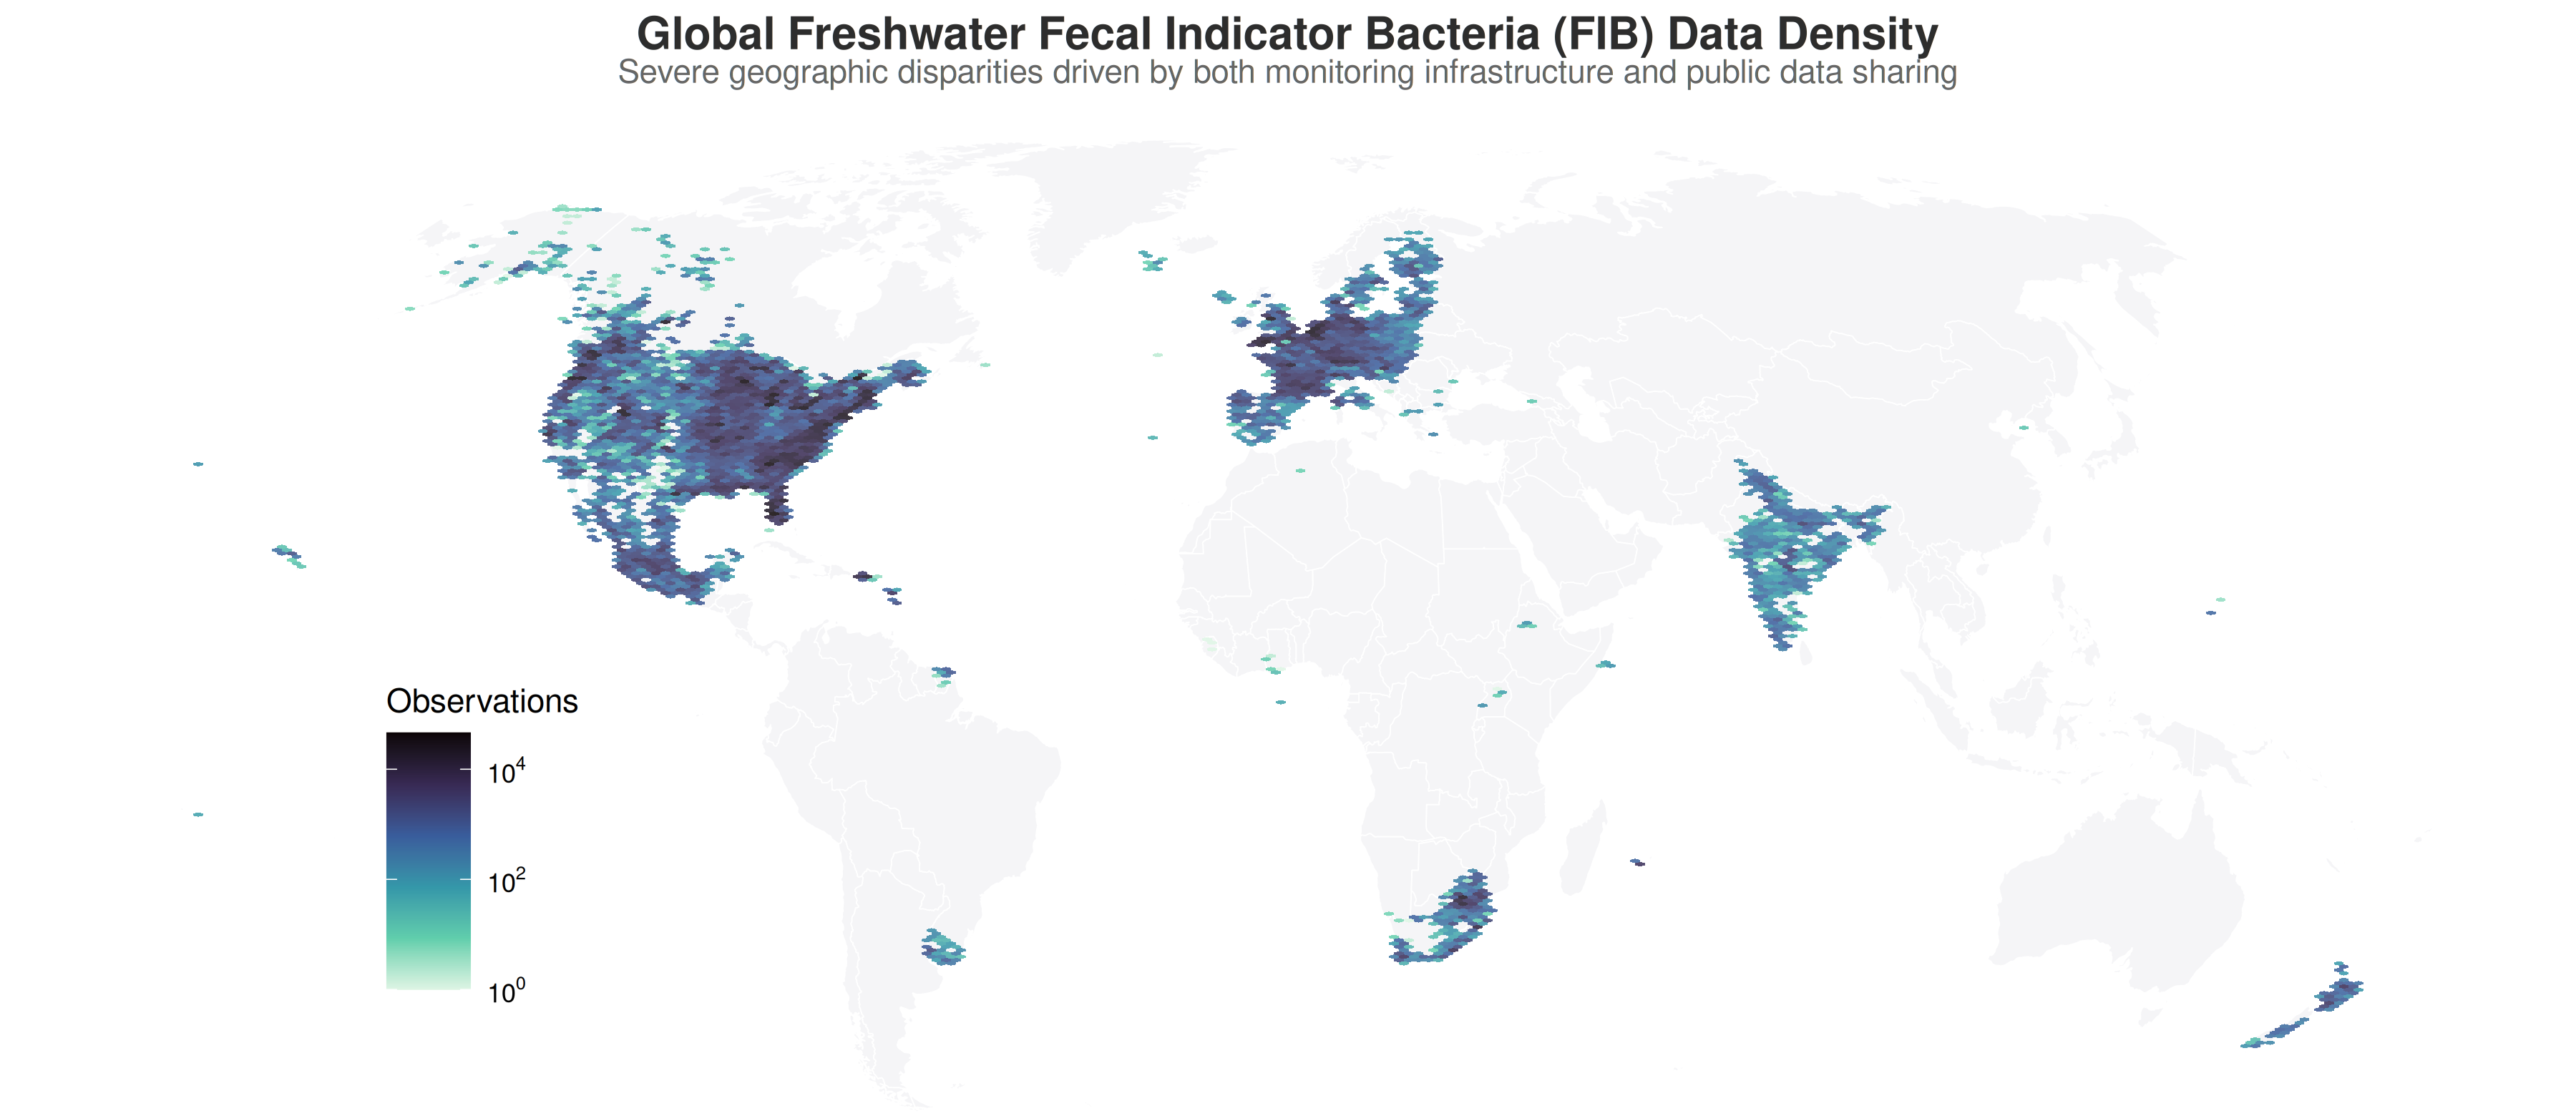
\includegraphics[width=\textwidth]{fig_global_distribution_density.png}
\caption{Global density of freshwater fecal indicator bacteria observations on a Robinson projection, aggregated into hexagonal bins and shaded on a logarithmic scale, with an inset of observations by ecosystem class. Monitoring is concentrated in the United States and Europe, with sparse coverage across most of the Global South and an almost complete absence over Russia and China.}
\label{fig:distribution}
\end{figure}

\begin{table}
\caption{Geographic distribution of the freshwater analysis dataset.}
\centering
\begin{tabular}{l r r}
\hline
Region & Records & Share \\
\hline
United States & 3{,}342{,}758 & 62.9\% \\
Europe & 1{,}099{,}575 & 20.7\% \\
Canada & 305{,}432 & 5.7\% \\
Rest of world & 567{,}026 & 10.7\% \\
\hline
\end{tabular}
\label{tab:geography}
\end{table}

\subsection{Indicator and ecosystem composition}
No single indicator dominates the dataset: \textit{E. coli} accounts for 43.4\% of records, fecal coliform for 31.8\%, total coliform for 10.5\%, intestinal enterococci for 9.0\%, and fecal streptococci for 5.2\% (Table~\ref{tab:composition}). Coverage of non-\textit{E. coli} indicators is uneven across sources; intestinal enterococci, for example, derive almost entirely from European inland bathing waters. By ecosystem, the data are dominated by rivers and streams (72.4\%) and lakes (22.6\%), with reservoirs, canals, ditches, springs, wetlands, and ponds making up the remainder.

\begin{table}
\caption{Indicator and ecosystem composition of the freshwater dataset.}
\centering
\begin{tabular}{l r r}
\hline
Category & Records & Share \\
\hline
\textit{E. coli} & 2{,}308{,}643 & 43.4\% \\
Fecal coliform & 1{,}692{,}665 & 31.8\% \\
Total coliform & 560{,}355 & 10.5\% \\
Intestinal enterococci & 479{,}053 & 9.0\% \\
Fecal streptococci & 274{,}075 & 5.2\% \\
\hline
River or stream & 3{,}848{,}418 & 72.4\% \\
Lake & 1{,}199{,}766 & 22.6\% \\
Other freshwater & 266{,}607 & 5.0\% \\
\hline
\end{tabular}
\label{tab:composition}
\end{table}

\subsection{The actionability gap in sampling frequency}
Most sites are sampled too sparsely, and too infrequently, to resolve transient contamination (Figure~\ref{fig:actionability}). Of 133{,}328 distinct sites, only 10.8\% have at least 100 observations and just 0.7\% have at least 500. Among the 116{,}489 sites with two or more samples, only 7.0\% are sampled at a daily or near-daily cadence, whereas 29.9\% are sampled monthly and 30.7\% quarterly (Table~\ref{tab:intervals}). The contrast in monitoring objectives is illustrated in Figure~\ref{fig:objectives}, which compares three Wisconsin sites whose designs differ by an order of magnitude in sampling frequency.

\begin{figure}
\noindent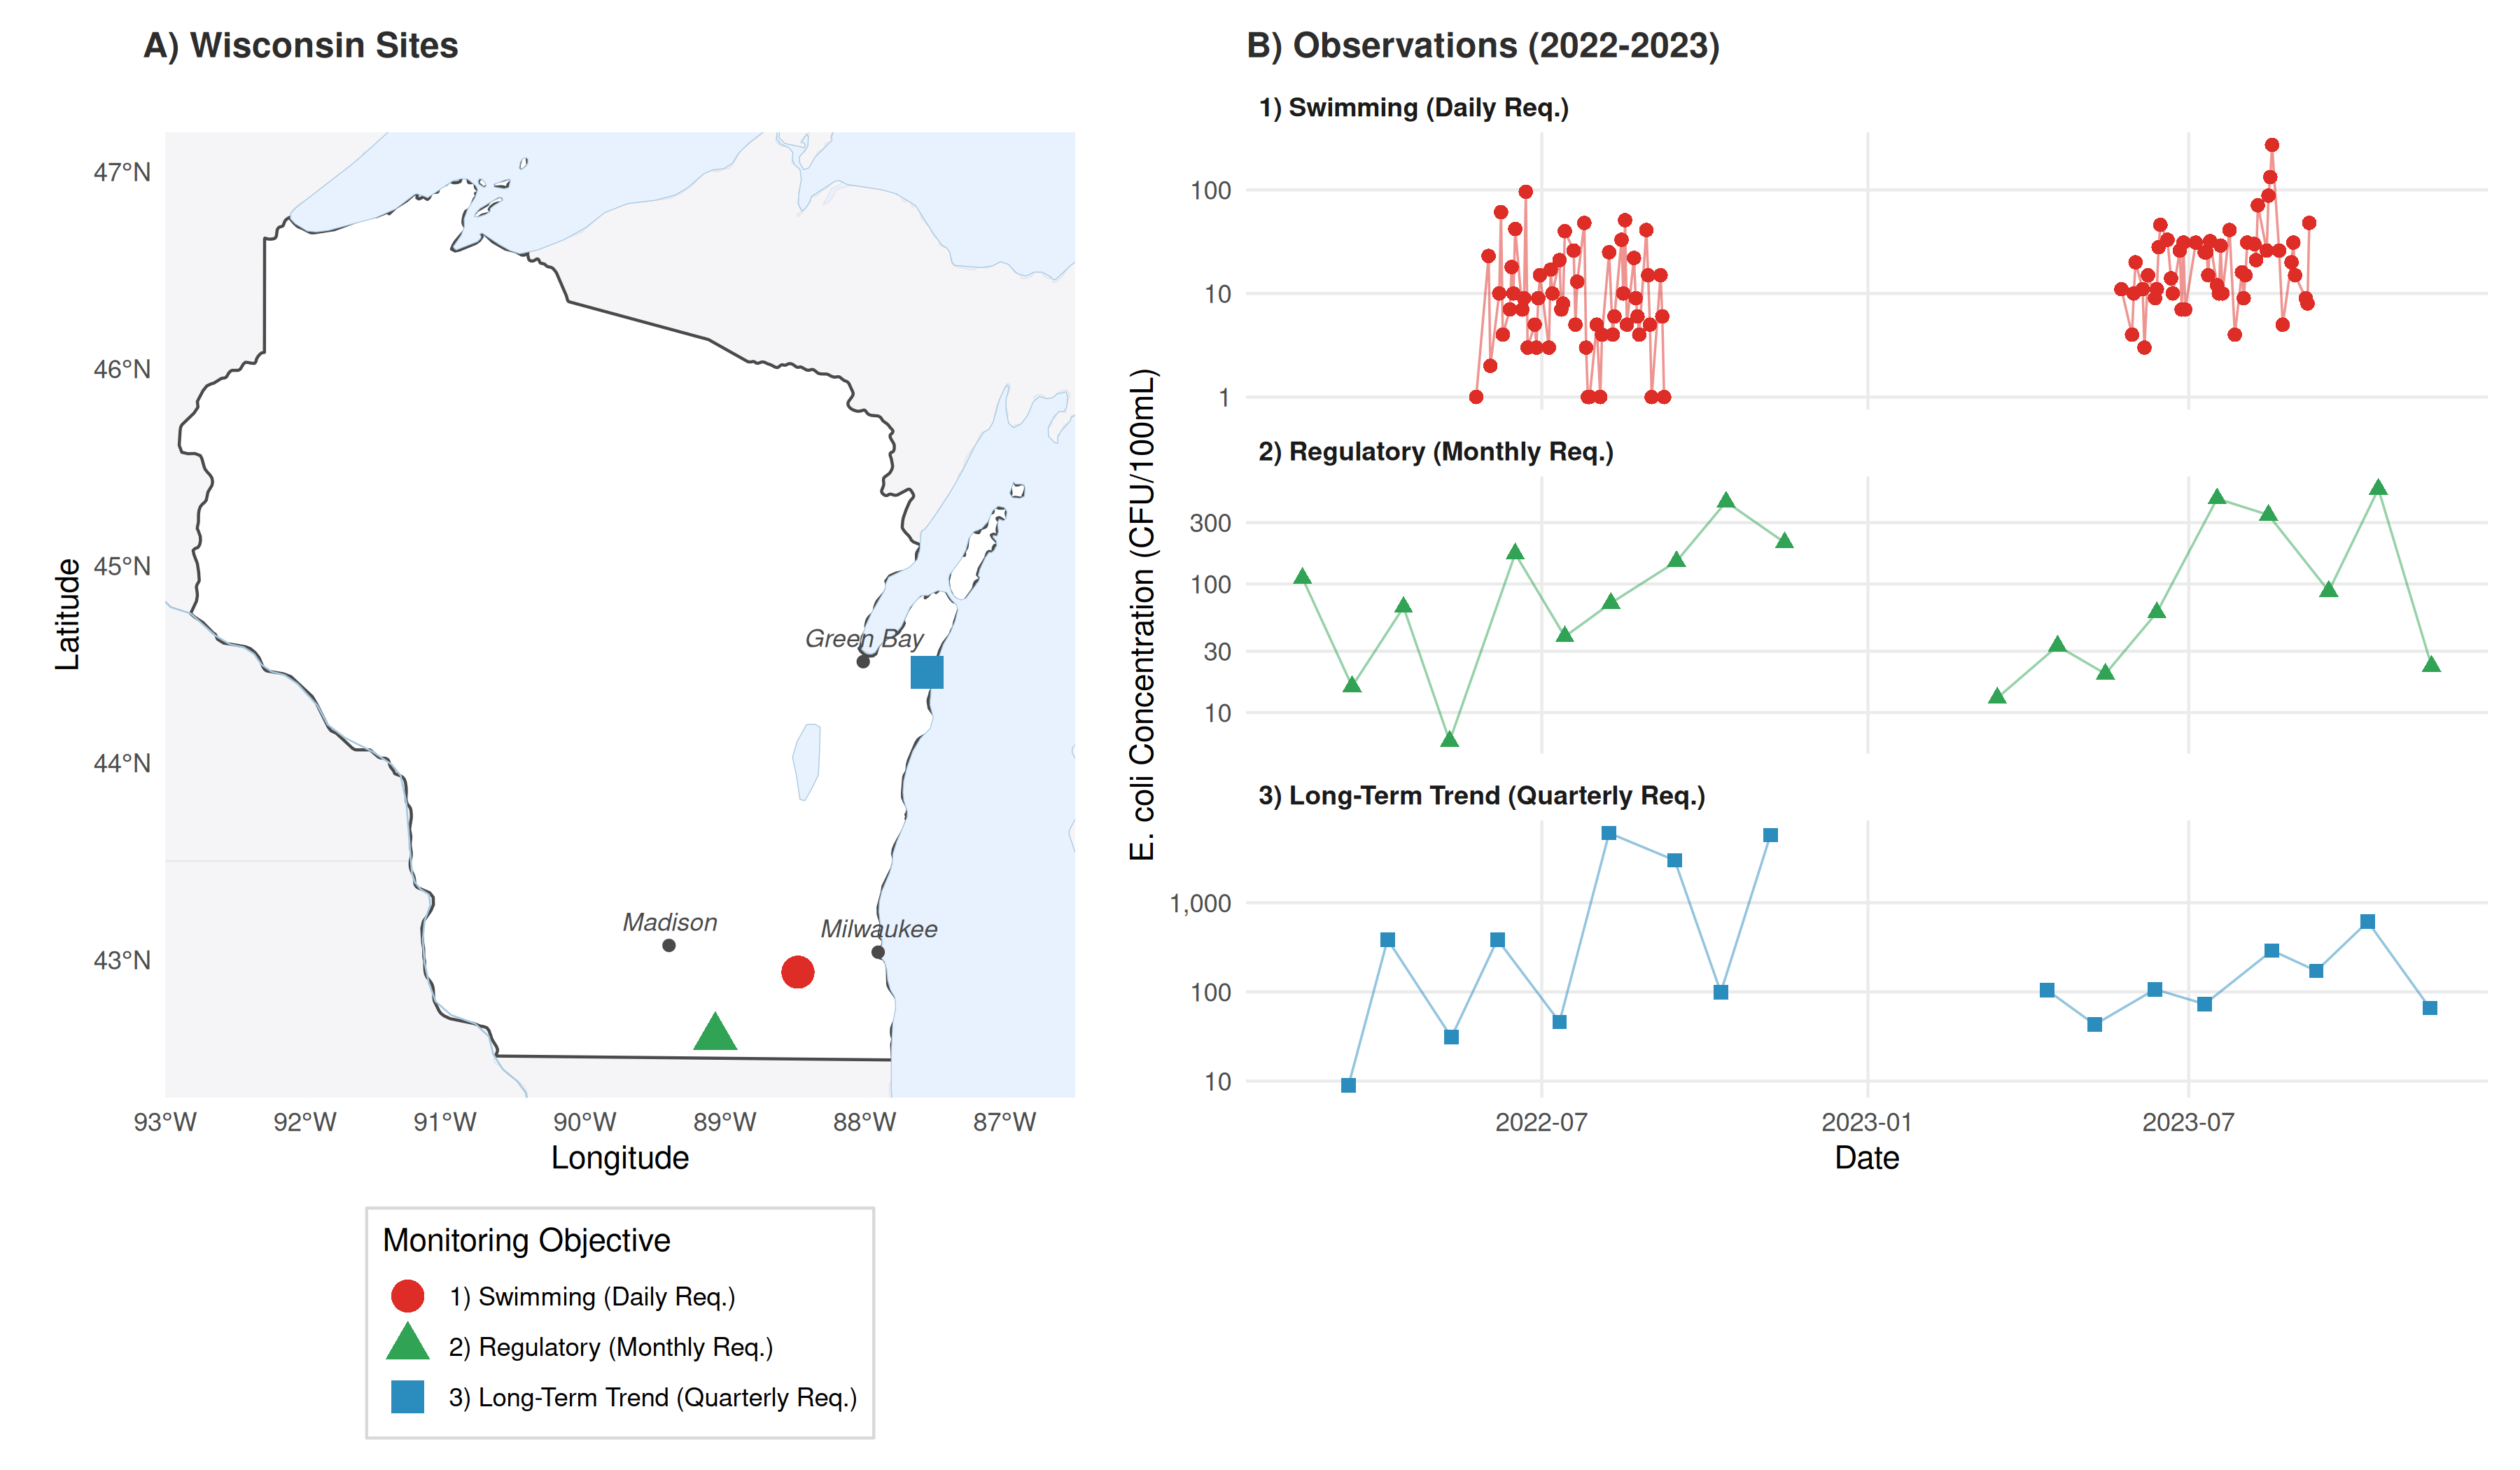
\includegraphics[width=\textwidth]{fig_sampling_frequency_mismatch.png}
\caption{Three Wisconsin freshwater sites with contrasting sampling cadences. The locator map marks a daily-sampled swimming beach, a monthly regulatory river site, and a quarterly trend site; the panels show their 2022--2023 \textit{E. coli} observations, with 101, 19, and 17 samples respectively. Sampling frequency, rather than concentration trend, distinguishes the three designs.}
\label{fig:objectives}
\end{figure}

\begin{figure}
\noindent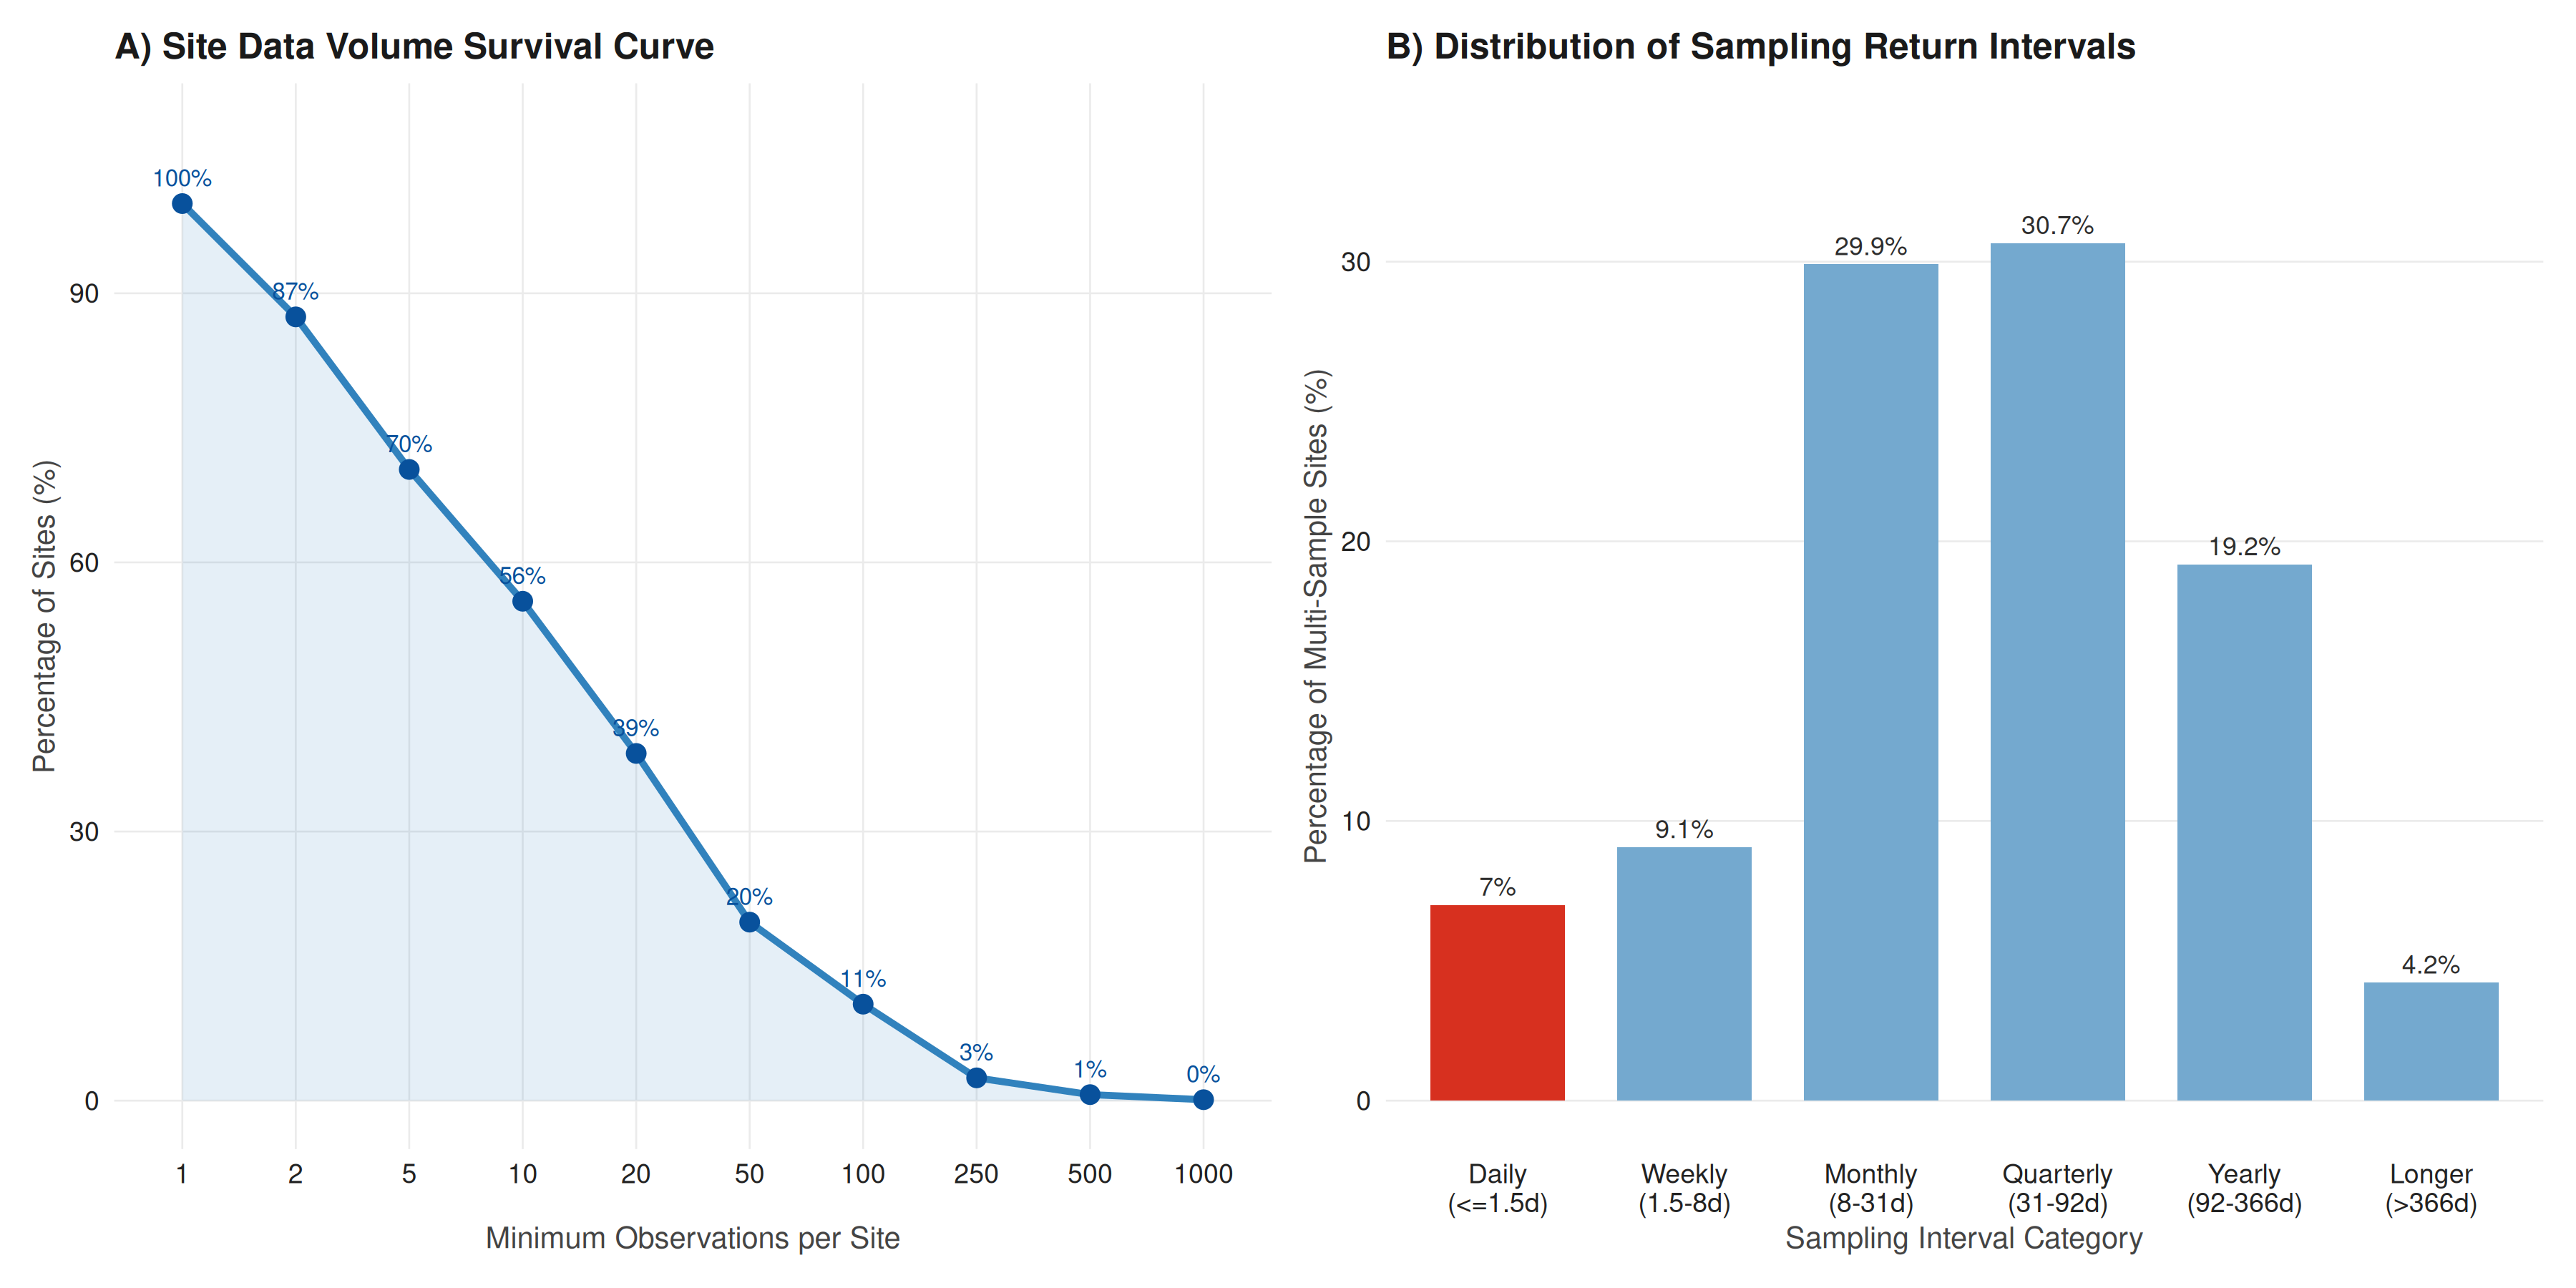
\includegraphics[width=\textwidth]{fig_actionability_gap.png}
\caption{Quantifying the actionability gap. Left: the percentage of sites retained as the minimum observation count per site increases. Right: the distribution of mean sampling return intervals among multi-sample sites, with the near-daily category highlighted.}
\label{fig:actionability}
\end{figure}

\begin{table}
\caption{Distribution of per-site sampling return intervals among the 116{,}489 sites with at least two samples.}
\centering
\begin{tabular}{l r}
\hline
Return interval band & Share of multi-sample sites \\
\hline
Daily (at most 1.5 days) & 7.0\% \\
Weekly (1.5 to 8 days) & 9.1\% \\
Monthly (8 to 31 days) & 29.9\% \\
Quarterly (31 to 92 days) & 30.7\% \\
Yearly (92 to 366 days) & 19.2\% \\
Longer (over 366 days) & 4.2\% \\
\hline
\end{tabular}
\label{tab:intervals}
\end{table}

\subsection{High-frequency safety and case studies}
High-frequency monitoring is rare and geographically concentrated in North America and Europe (Figure~\ref{fig:safety}). Across 631 high-frequency sites comprising 235{,}398 \textit{E. coli} samples, 77.6\% of observations were at or below the safe threshold and 22.4\% exceeded it, but per-site exceedance rates vary widely, from sites that are consistently safe to sites in agricultural or urban catchments that are chronically above the threshold. The three 2023 case studies in Figure~\ref{fig:casestudies} and Table~\ref{tab:cases} make the implication concrete: an enclosed Lake Erie beach in the United States was safe most of the time (18.0\% exceedance) with short-lived spikes that recovered within days, whereas the River Lune in the United Kingdom and the Taruheru River in New Zealand exceeded the safe threshold for the majority of the year (83.7\% and 62.5\% exceedance). In the first case, a single monthly grab sample taken during a transient spike would have closed an otherwise-safe beach for weeks; in the latter two, a favorably timed monthly sample could have certified as safe a river that was unsafe most of the year. Low-frequency sampling therefore misrepresents safety in both regimes, and higher-frequency data improve management in both.

\begin{figure}
\noindent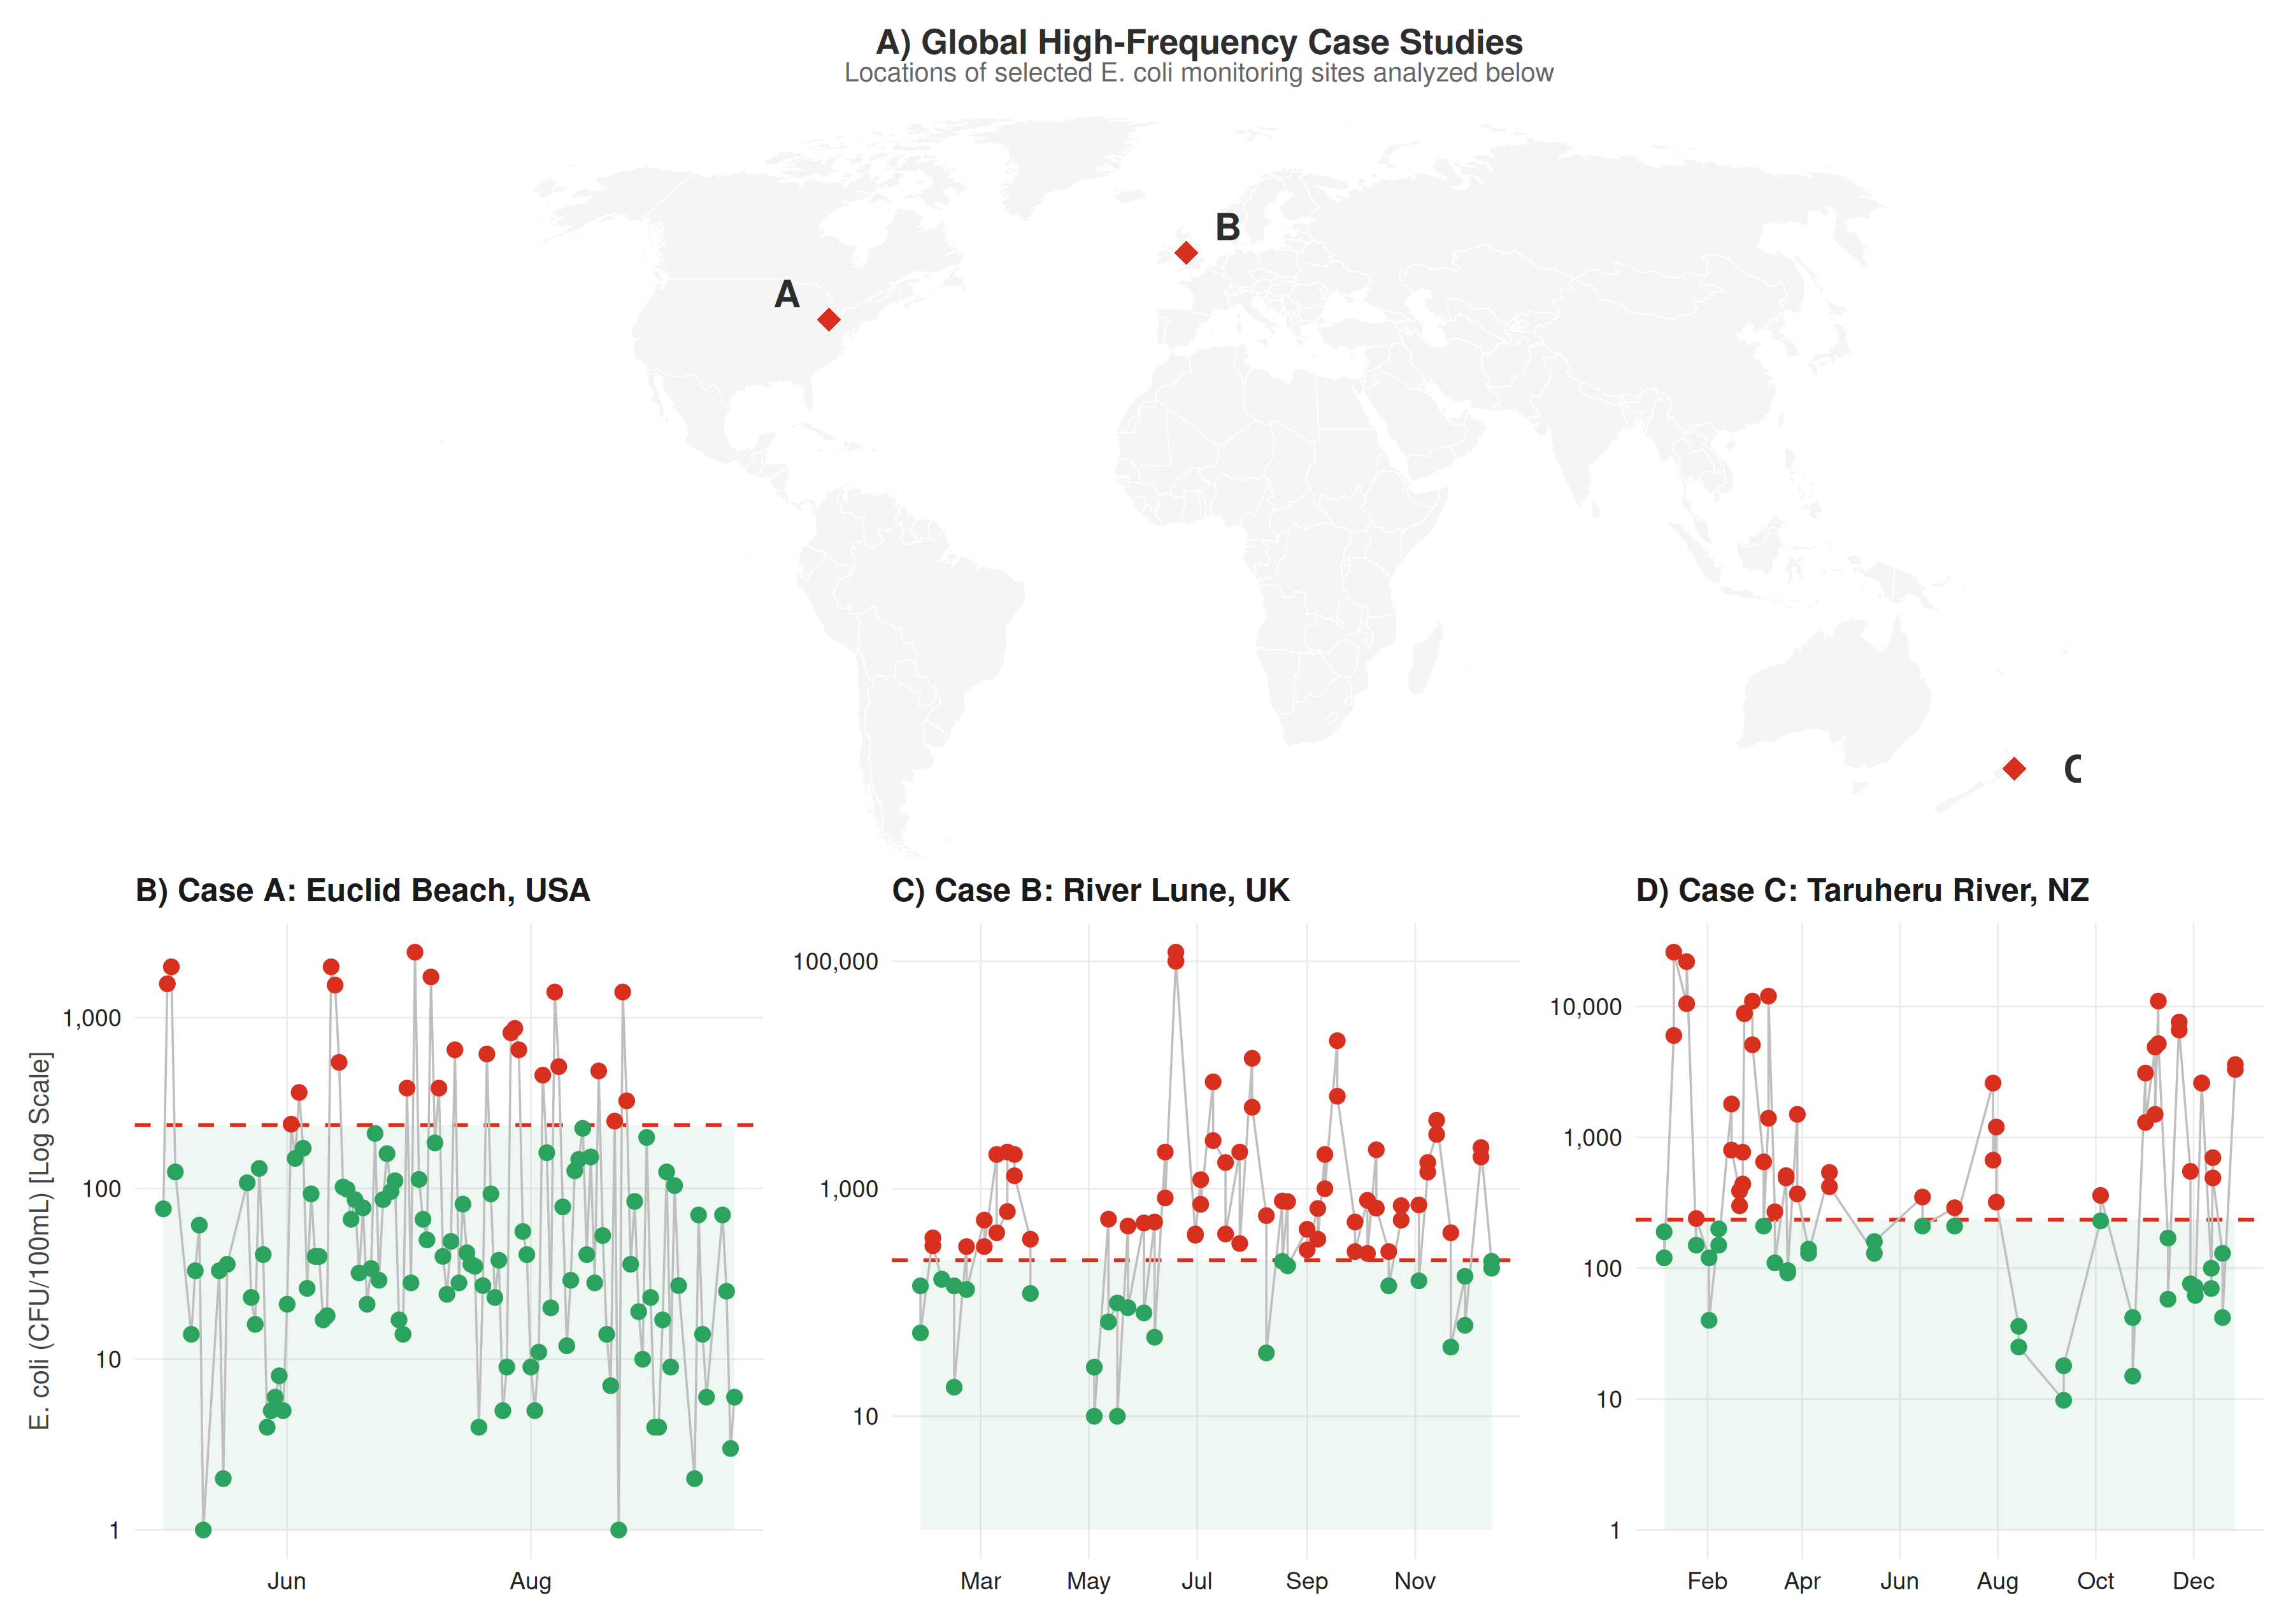
\includegraphics[width=\textwidth]{fig_high_frequency_case_studies.png}
\caption{High-frequency \textit{E. coli} monitoring at three sites on three continents in 2023, plotted against the 235 colony forming units per 100~mL safe threshold with a shaded safe zone. The Lake Erie beach (United States) remained largely safe with short-lived spikes, whereas the River Lune (United Kingdom) and Taruheru River (New Zealand) exceeded the threshold for most of the year.}
\label{fig:casestudies}
\end{figure}

\begin{figure}
\noindent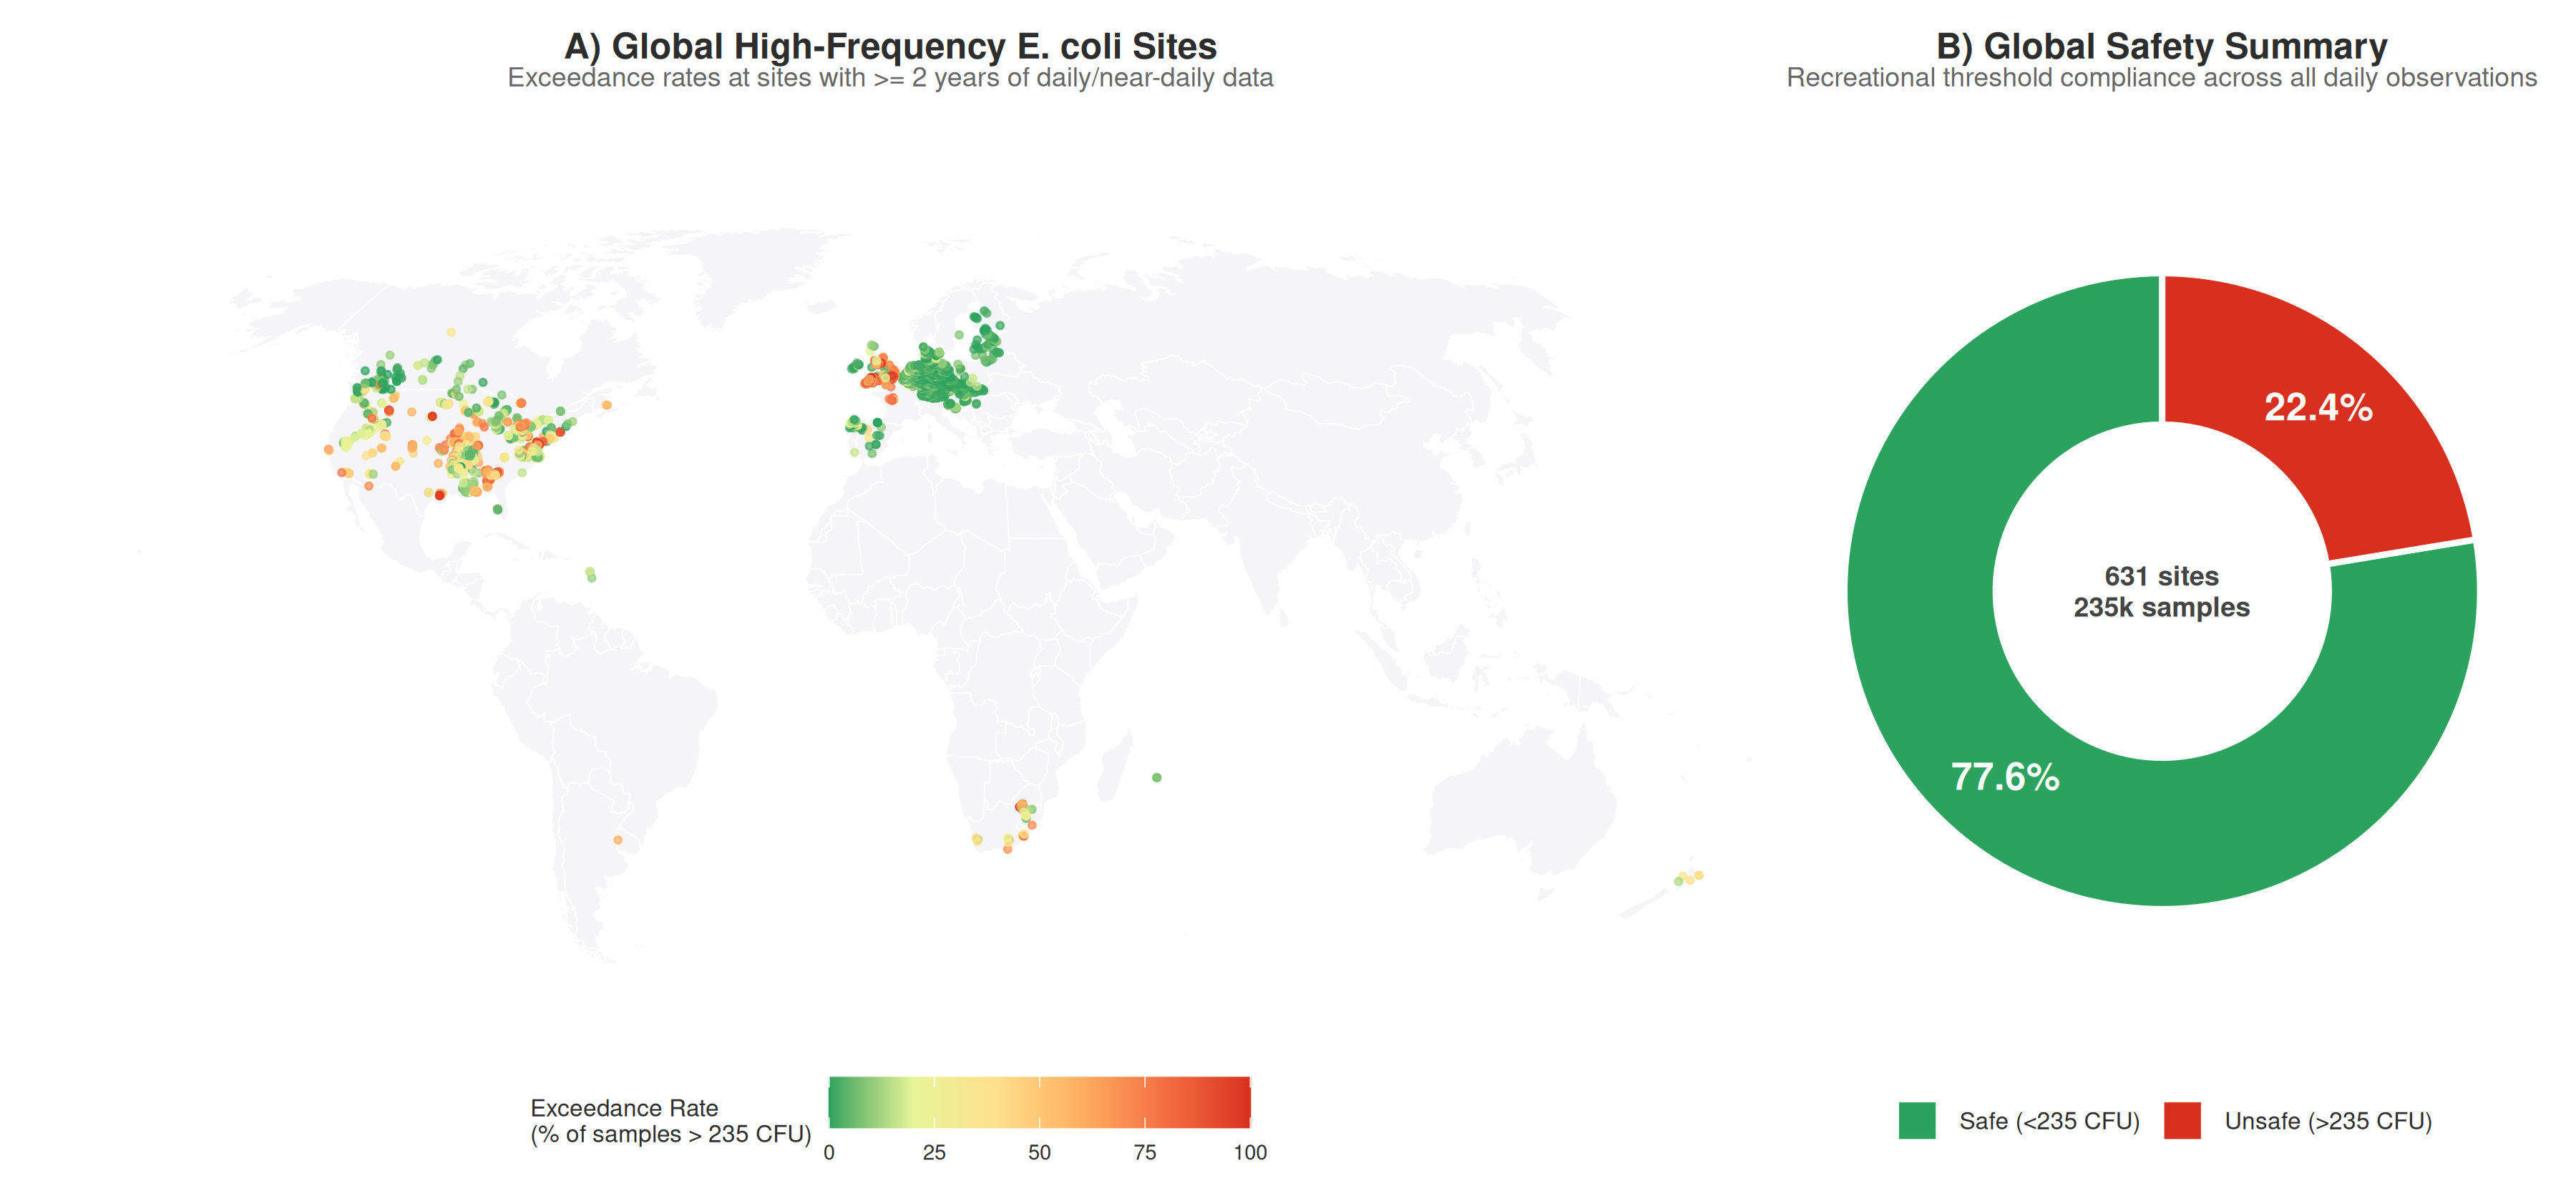
\includegraphics[width=\textwidth]{fig_global_safety_summary.png}
\caption{Global safety of high-frequency \textit{E. coli} monitoring sites. The map plots sites with at least near-daily sampling, colored by the share of samples exceeding the safe threshold; the donut summarizes the overall split of 77.6 percent safe versus 22.4 percent unsafe across 631 sites and 235{,}398 samples.}
\label{fig:safety}
\end{figure}

\begin{table}
\caption{High-frequency case-study sites in 2023.}
\centering
\begin{tabular}{l l r r r r}
\hline
Site & Country & Samples & Exceedance & Median & Maximum \\
\hline
Euclid Beach & United States & 128 & 18.0\% & 41 & 2{,}420 \\
River Lune & United Kingdom & 43 & 83.7\% & 580 & 100{,}000 \\
Taruheru River & New Zealand & 40 & 62.5\% & 465 & 11{,}000 \\
\hline
\multicolumn{6}{l}{$^a$ Median and maximum concentrations in colony forming units per 100~mL.}
\end{tabular}
\label{tab:cases}
\end{table}

\section{Discussion}

\subsection{Collection gap versus sharing gap}
The geography of the freshwater record (Figure~\ref{fig:distribution}) is best understood as the joint product of two distinct gaps. A genuine collection gap exists in resource-limited regions where monitoring capacity is constrained and varies with national development \cite{kirschke2020capacity}. But the near-absence of large, industrialized monitoring nations from the open record points to a second, sharing gap: data are collected but not published in open, machine-readable, harmonized form. This interpretation is consistent with a literature documenting persistent technical, institutional, and social barriers to sharing environmental and water-quality data \cite{brasier2017barriers,sugg2021social,hazell2023sociotechnical,heacock2022enhancing,kumpel2020data}, and it implies that funding new stations alone will not close the gap. Wider adoption of the FAIR principles \cite{wilkinson2016fair}, together with data-sharing norms comparable to those that govern international exchange of meteorological data, would convert existing but invisible monitoring into a usable global resource.

\subsection{Regulatory rigidity and management implications}
Our cadence results quantify a mismatch between how fecal indicators are monitored and how they behave. Because contamination is transient \cite{whitman2004escherichia,traister2006variability,meays2006diurnal}, calendar-based low-frequency sampling is structurally blind to acute risk, and because culture-based assays return results only after roughly a day, advisories are inherently retrospective \cite{kim2004public}. The high-frequency case studies show that this rigidity cuts both ways: infrequent sampling can both over-restrict an otherwise-safe beach after a single spike and certify as safe a chronically polluted river. Higher-frequency, event-based sampling, and predictive nowcasting models that exploit rainfall, turbidity, and discharge \cite{searcy2021day,searcy2023highfrequency,heasley2021systematic}, therefore offer substantial gains in both directions. Scaling such approaches beyond the handful of intensively studied sites we identify is, in our view, the central operational opportunity.

\subsection{Limitations}
Several limitations bound our conclusions. The treatment of most-probable-number values as colony forming units is an approximation, and datetimes and time zones were not harmonized globally. Coverage of non-\textit{E. coli} indicators is uneven across sources, so cross-indicator comparisons of total monitoring effort should be made cautiously. High-frequency sites are geographically biased toward North America and Europe, so the 77.6\% safe fraction is conditional on those sites and is not a globally representative safety rate. Finally, the case studies are individual sites chosen to illustrate distinct regimes rather than a representative sample.

\section{Conclusions}
We assembled and characterized the first harmonized, global, freshwater-focused dataset of fecal indicator bacteria, comprising 5{,}314{,}791 observations from ten public sources. The record exhibits two structural weaknesses for public health: a spatial concentration of openly shared data in a few wealthy regions that reflects an open-data sharing barrier as much as a collection gap, and a temporal rigidity in which only a small minority of sites are sampled often enough to resolve the transient dynamics of fecal contamination. High-frequency sites demonstrate that low-frequency monitoring misrepresents safety in both episodically and chronically contaminated waters. Closing these gaps will require both open, FAIR data sharing and a shift toward higher-frequency, event-based, and predictive monitoring.

\section*{Open Research Section}
The harmonized freshwater fecal indicator dataset and the data-cleaning and figure-generation code that support the findings of this study will be archived in a public repository with a persistent identifier prior to publication [repository DOI --- to be completed]; data are not available solely from the authors. The underlying observations were obtained from the following public sources, each of which should be cited in the final reference list with its access point: the US Water Quality Portal \cite{read2017water}, the European Environment Agency Eionet bathing-water reporting system, the UN GEMS/Water GEMStat database, DataStream, the UK Environment Agency Water Quality Archive, the South African National Microbial Monitoring Programme, the French Hub'Eau Naiades service, Land Air Water Aotearoa, the Water Point Data Exchange, and the Brazilian National Water Agency. [Per-source data citations with persistent identifiers to be completed.]

\section*{Conflict of Interest disclosure}
The authors declare no conflicts of interest for this manuscript.

\acknowledgments
[Funding sources and acknowledgments to be completed.]

\bibliography{refs}

\end{document}
